% \section{Background}
\section{Antecedentes}

% =====================================
% RESULTADOS DEL SEMESTRE ANTERIOR
%   - Usamos el método de Imputación Mendeliana para 17 rasgos complejos.
%   - Nos dimos cuenta que, si bien el workflow de snipar funciona, la imputación mendeliana
%   no es adecuada para poblaciones mestizas como México.
% =====================================

% \begin{frame}[c]{Incrementar Tamaño de Muestra: Imputación Mendeliana}
%     \begin{columns}
%         % --- Mendelian Imputation ---
%         \begin{column}{0.65\textwidth}
%             \begin{figure}
%                 \centering
%                 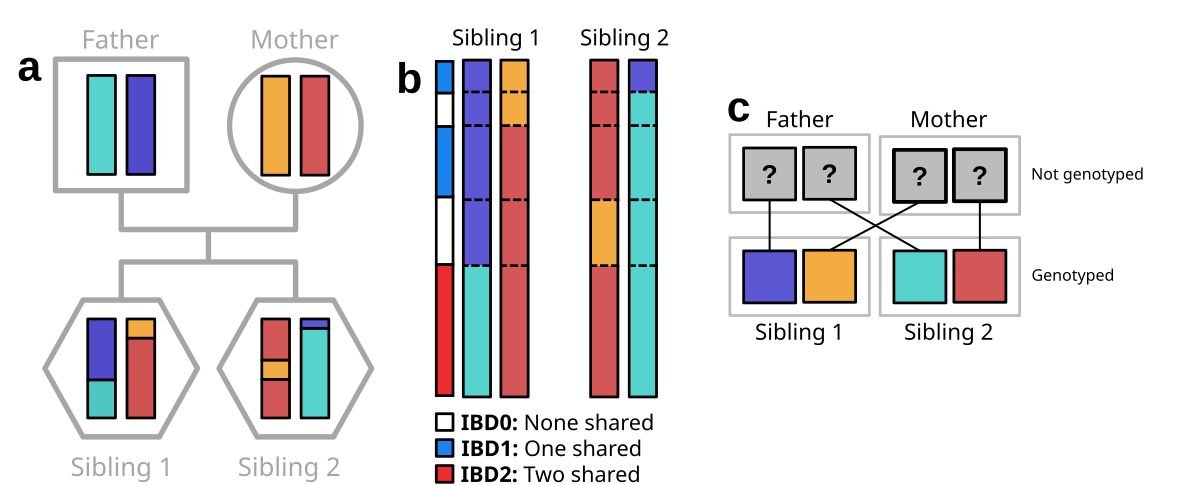
\includegraphics[width=0.9\textwidth]{img/diagrams/mendelian-imputation.png} 
%                 \caption{
%                     \textbf{El proceso de meisosis segrega aleatoriamente los alelos parentales.}
%                     (A)
%                     (B)
%                 }
%             \end{figure}
%         \end{column}
% 
%         % --- Manhattan Plot of previous results ---
%         \begin{column}{0.35\textwidth}
%             \sffamily\centering
%             \only<2->{
%                 {\small
%                     La \enquote{Imputación mendeliana} \parencite{young2022-fgwas} \textbf{introduce sesgos} en poblaciones con \textbf{mestizaje reciente}.\\[2.5pt]
%                 }
%                 {\scriptsize
%                     \textcolor{gray}{Depende de \textit{frecuencias alélicas} para algunos casos de IBD.}\\[2em]
%                 }
%             }
%             \only<3->{\small
%                 \alert{No podemos confiar} en asociaciones que usen \enquote{Imputación mendeliana} en el MCPS.\\[1em]
%             }
%             \only<4->{\small
%                 ¿Cómo incrementamos el tamaño de muestra de forma \textbf{robusta} al mestizaje reciente?
%             }
%         \end{column}
%     \end{columns}
% \end{frame}

% ============================================================
% Robust estimator
% ============================================================
% \begin{frame}[c]{Incrementar Tamaño de Muestra: Estimador robusto}
%   \begin{columns}[b]
%     % --- LEFT COLUMN: Traditional methods ---
%     \begin{column}{0.45\textwidth}
%       \centering
%       {\footnotesize
%         % Traditional methods like \textcite{benyamin2009-fgwas,howe2022-sibdiff,young2022-fgwas}.
%         Métodos de FGWAS convencionales \parencite{benyamin2009-fgwas,howe2022-sibdiff,young2022-fgwas}.
%       }\\[1.5em]
%       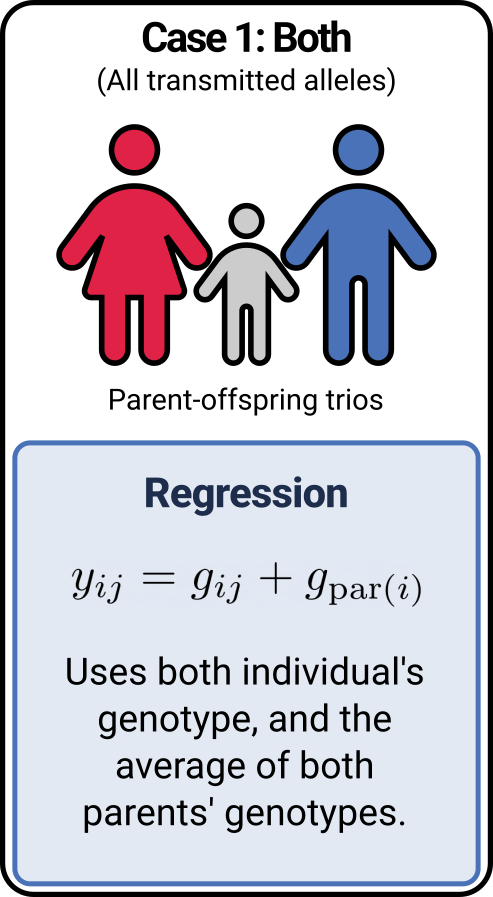
\includegraphics[height=4cm]{img/diagrams/robust-estimator/case-01.png}
%       
%       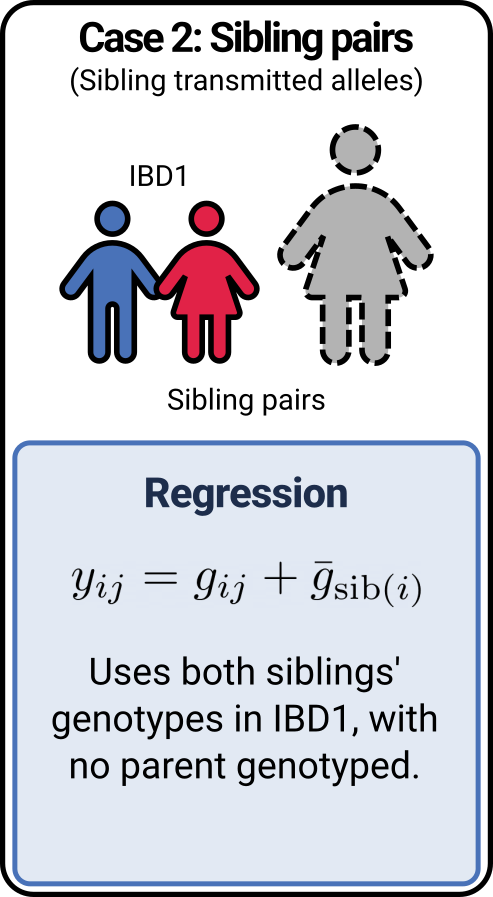
\includegraphics[height=4cm]{img/diagrams/robust-estimator/case-02.png}
%     \end{column}
% 
%     \pause
% 
%     % --- RIGHT COLUMN: Robust estimator ---
%     \begin{column}{0.45\textwidth}
%       \centering
%       %
%       {\footnotesize
%         % The \textit{robust estimator} by \textcite{guan2025-fgwas} \textbf{increases} effective sample size ($N_{\mathrm{eff}}$) and it is robust to \textbf{recent admixture}.
%         El \enquote{estimador robusto} \parencite{guan2025-fgwas} \textbf{incrementa} el tamaño efectivo de muestra, siendo robusto a \textit{mestizaje reciente}.
%       }\\[1.5em]
%       %
%       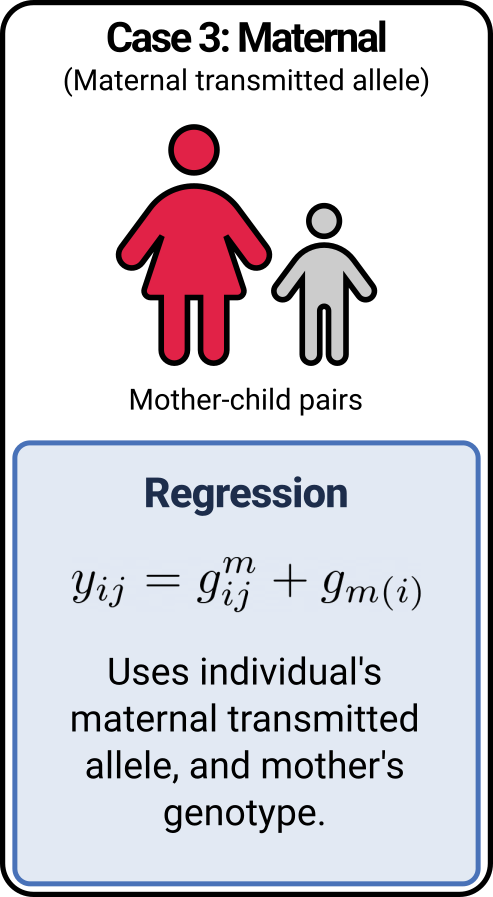
\includegraphics[height=4cm]{img/diagrams/robust-estimator/case-03.png}
%       \hspace{1em}
%       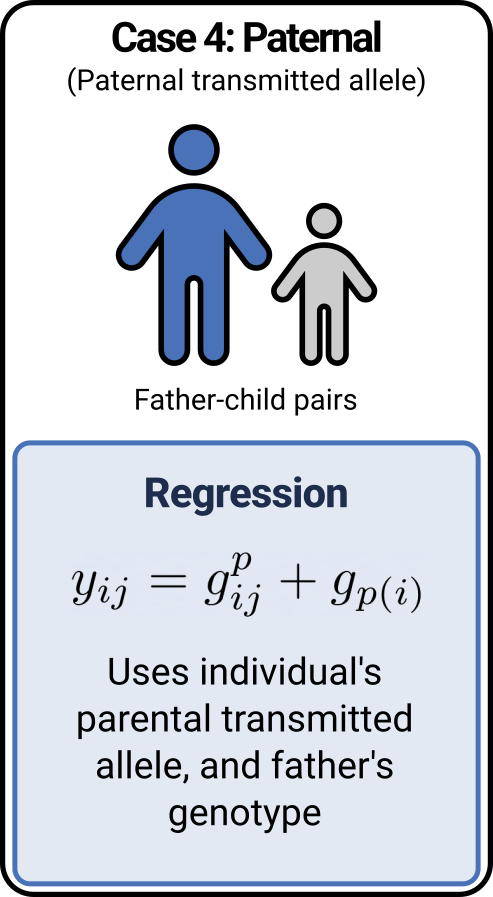
\includegraphics[height=4cm]{img/diagrams/robust-estimator/case-04.png}
%     \end{column}
%   \end{columns}
% \end{frame}

\begin{frame}[c]{Incrementando poder estadístico: Estimador robusto}
    \vspace{1em}
    \begin{columns}[c]
        % --- Column A ----
        \begin{column}{0.35\textwidth}
            \textbf{Cambio de estrategia...}\\[1em]
            \footnotesize
            \begin{itemize}
                \item<1-> La \textit{Imputación Mendeliana} \parencite{young2022-fgwas} es sensible a \textbf{frecuencias alélicas}.
                \item<2-> En cohortes con mestizaje reciente ---como el MCPS--- la \textit{Imputación Mendeliana} puede introducir sesgos.
                \item<3-> El \textit{Estimador Robusto} de \textcite{guan2025-fgwas} expande el tamaño de muestra para FGWAS, siendo robusto a mestizaje reciente.
            \end{itemize}
        \end{column}

        % --- Column B ----
        \begin{column}{0.70\textwidth}<4->
            \centering
            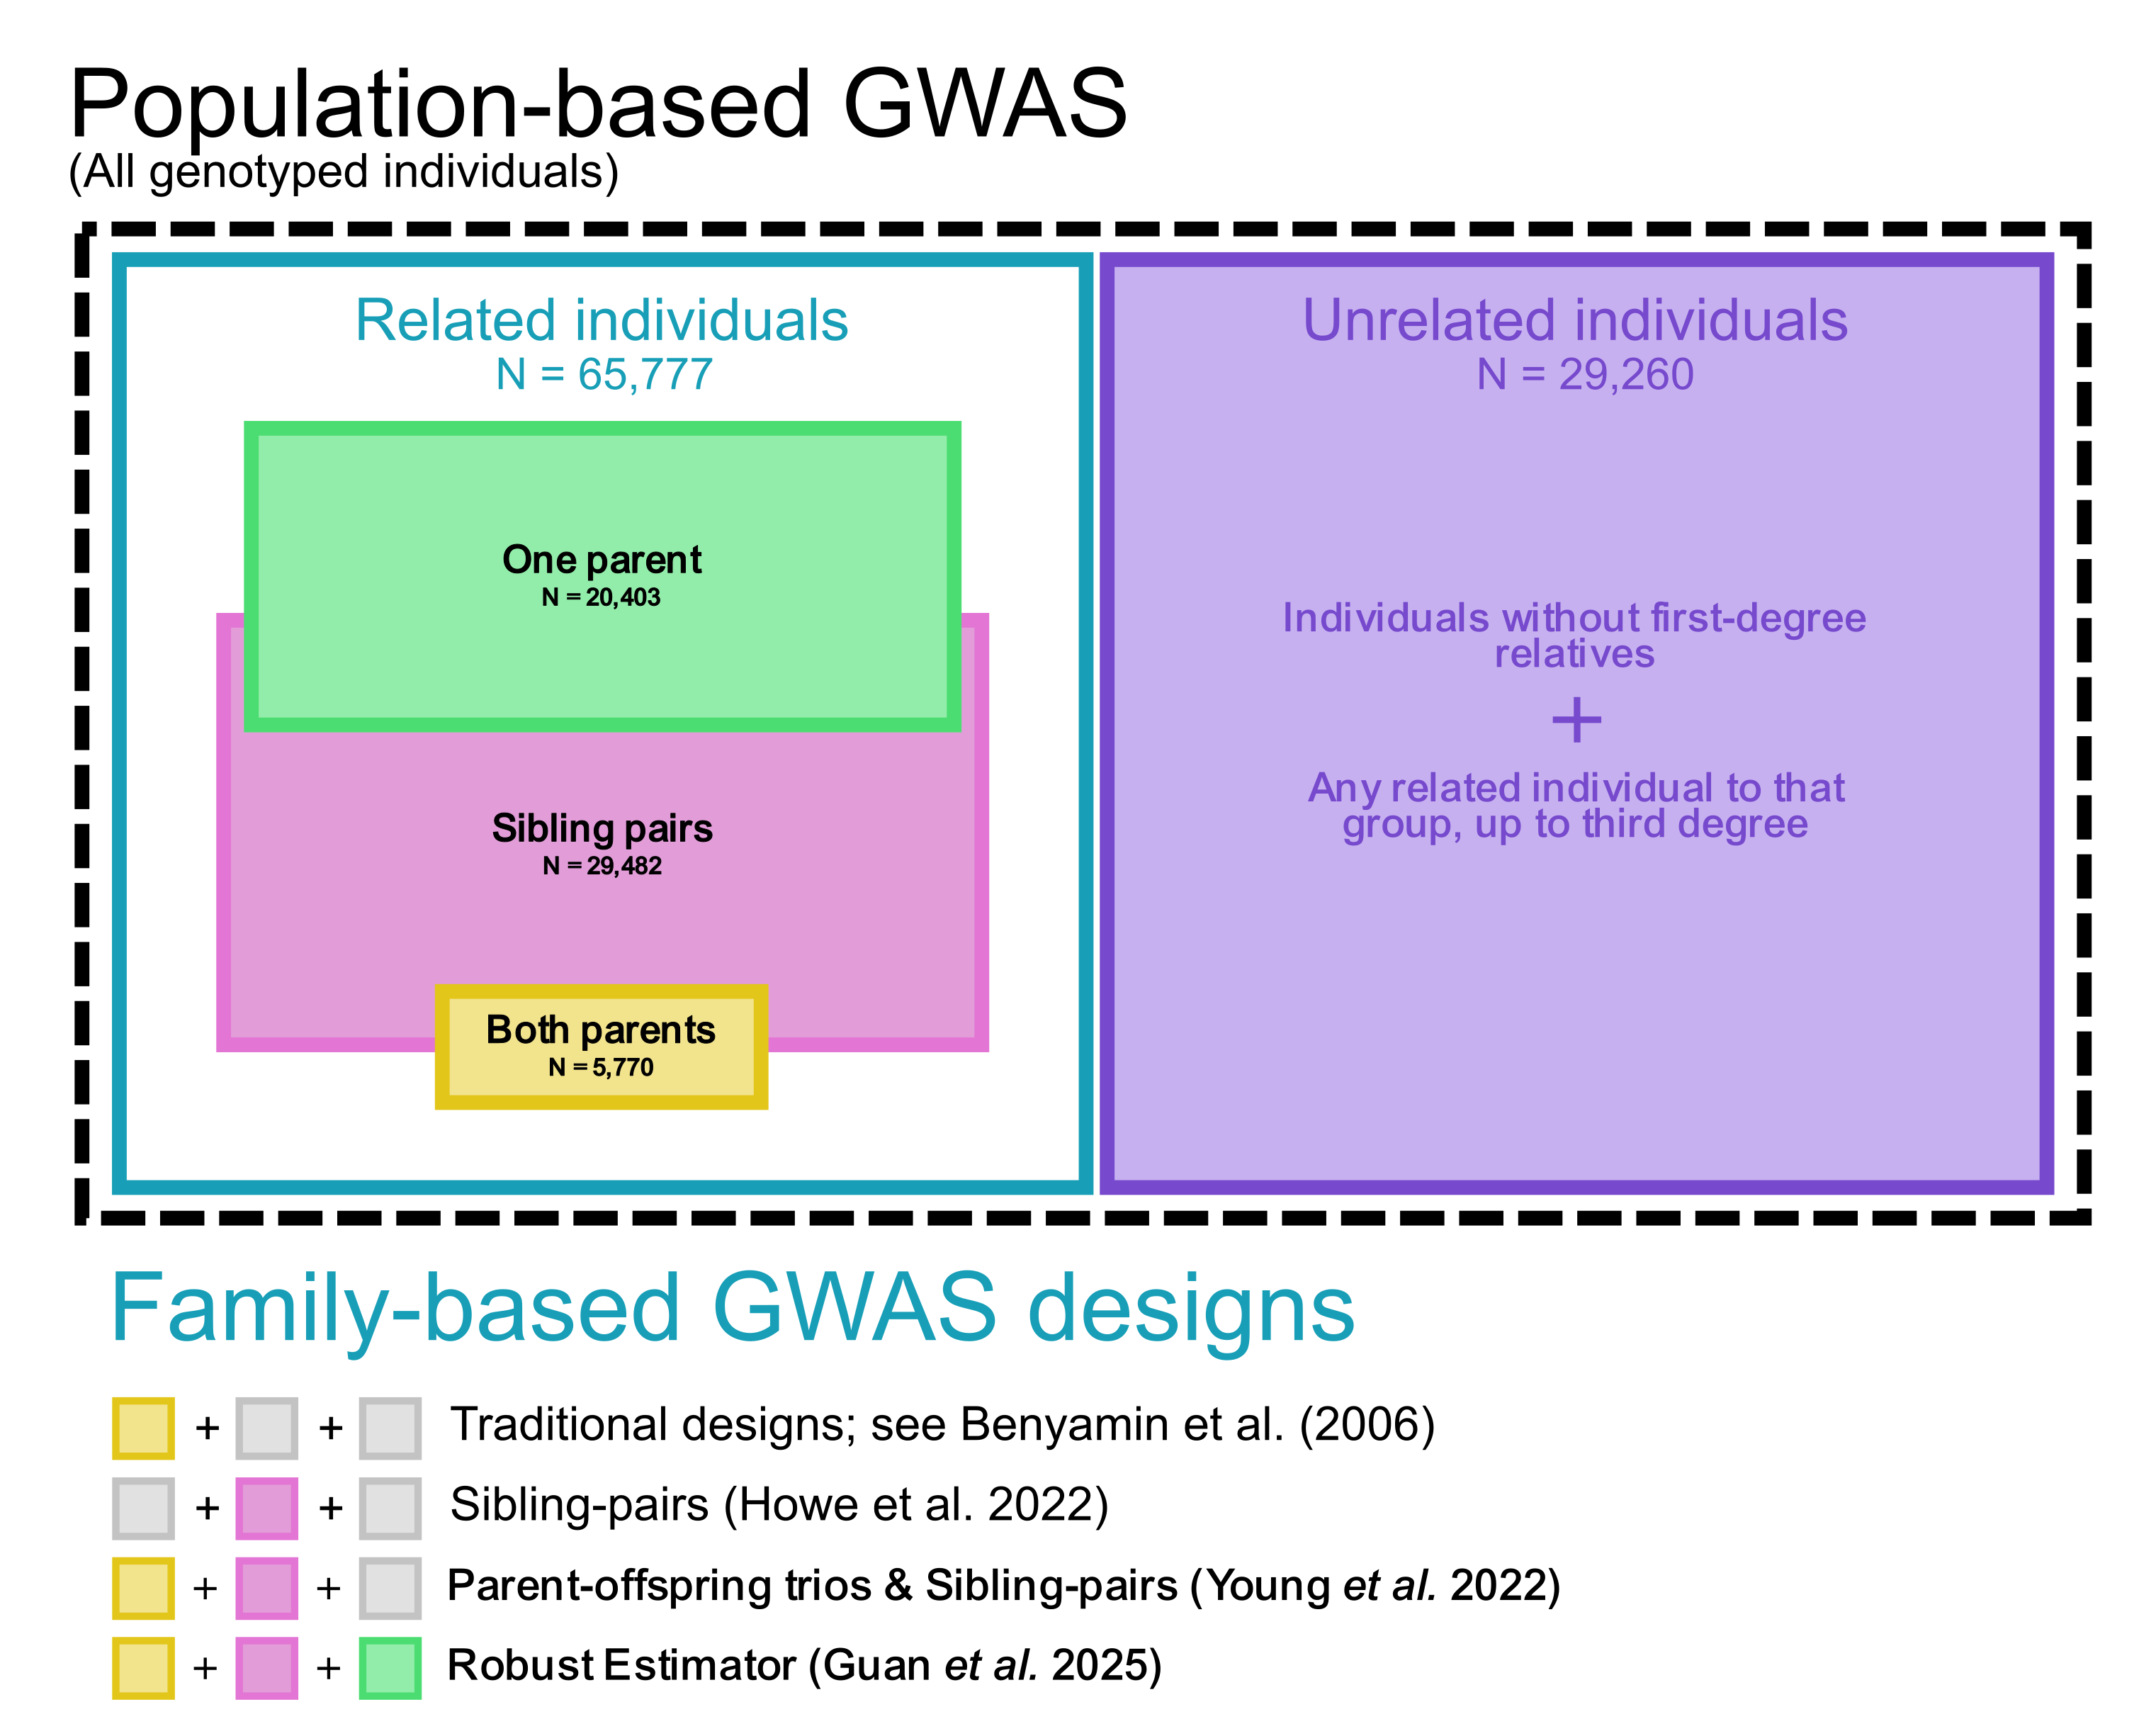
\includegraphics[width=0.80\textwidth]{img/diagrams/robust-estimator_neff.png}
        \end{column}
    \end{columns}
\end{frame}